\documentclass[11pt, a4paper]{article}
\usepackage{CJKutf8}
\usepackage{amsthm}
\usepackage{ulem}
\usepackage{xcolor}
\usepackage{amsmath}
\usepackage{amssymb}
\usepackage{courier}
\usepackage{geometry}
\usepackage{enumitem}
\usepackage{graphicx}
\usepackage{listings}
\usepackage{algorithm}
\usepackage{algorithmic}
\usepackage{indentfirst}
%\usepackage{float}
\usepackage[perpage,stable]{footmisc} 
\geometry{left=2.7cm, right=2.7cm, top=3cm, bottom=3cm}


\usepackage{graphics}

\usepackage[colorlinks,linkcolor=black,anchorcolor=blue,citecolor=green,
  %	CJKbookmarks=true,
]{hyperref}
\hypersetup{unicode}

\linespread{1.4}
\usepackage{indentfirst}
\setlength{\parindent}{2em}
\hypersetup{hidelinks}

\usepackage{listings}
\lstset{
  numbers=left,
  texcl=true,
  escapechar=`,
  backgroundcolor=\color{lightgray!40!white}, 
  commentstyle=\rm\color{green!30!black},
  basicstyle=\footnotesize\tt,        % the size of the fonts that are used for the code
  breakatwhitespace=false,         % sets if automatic breaks should only happen at whitespace
  breaklines=true,                 % sets automatic line breaking
  captionpos=b,                    % sets the caption-position to bottom
  extendedchars=false,              % lets you use non-ASCII characters; for 8-bits encodings only, does not work with UTF-8
  frame=single,                    % adds a frame around the code
  language=Java,                 % the language of the code
  keywordstyle=\color{blue!70}\bfseries,
  showspaces=false,                % show spaces everywhere adding particular underscores; it overrides 'showstringspaces'
  showstringspaces=false,          % underline spaces within strings only
  showtabs=false,                  % show tabs within strings adding particular underscores
  tabsize=2                       % sets default tabsize to 2 spaces
}

\begin{document}
\begin{CJK*}{UTF8}{gbsn}
  \title{\bf Java程序“快速排序”设计报告}
  \author{马玉坤-1150310618}
  \date{2016年7月27日}
  \maketitle
  \renewcommand{\contentsname}{\textbf{目录}}
  \tableofcontents
  \newpage
  \newpage
  
  \section{题目描述}
  
  多线程编程编写一个龟兔赛跑程序。乌龟:速度慢,休息时间短;兔子:速度快,休息时间长。

  \section{总体设计思想}

  本实验中,我使用了继承自JLabel的类Runner来显示兔子和乌龟在休息或者奔跑时的图片。如果兔子在奔跑,显示run\_hare.jpg,否则显示stop\_hare.jpg。判断是否应该在休息,是通过类中的clocks变量。

  另一个类RaceThread实现了Runnable接口,用来构建窗口以及管理线程。

  最后,主类实例化RaceThread,执行RaceThread类的方法。

  \section{详细设计}

  \subsection{Runner类}

  \subsubsection{类声明}

  \begin{lstlisting}

class Runner extends JLabel {
  private int when_to_stop,  // 停止时的clocks值
    stop_time_length,        // 停止的时间长度
    px_in_one_step,          // 每50ms,x坐标的增量(像素)
    clocks,                  // 记录自线程运行开始的时间(t / 50ms)
    yc;                      // 该label的y坐标
  private ImageIcon img_run, // 奔跑时的ImageIcon
    img_stop;                // 停下休息时的ImageIcon
  public Runner(int _when_to_stop,
                int _stop_time_length,
                int _px_in_one_step,
                int _yc,
                ImageIcon _img_run,
                ImageIcon _img_stop);
  public void init();
  public void go();
}
    
  \end{lstlisting}
  
  \subsubsection{作用}

  继承自JLabel,根据线程运行所处的阶段调整label位置和label上的图片,用来显示兔子/乌龟在奔跑/休息。

  \lstinline$public void Runner::go()$方法按照当前的clocks值调整label的位置,以及根据clocks值调整label上的图片(奔跑或者休息)。

  \lstinline$public void Runner::init()$方法是将当前label初始化,初始化当前label的位置和大小。
  
  \subsubsection{类定义}
  \begin{lstlisting}
class Runner extends JLabel {
  private int when_to_stop,  // 停止时的clocks值
    stop_time_length,        // 停止的时间长度
    px_in_one_step,          // 每50ms,x坐标的增量(像素)
    clocks,                  // 记录自线程运行开始的时间(t / 50ms)
    yc;                      // 该label的y坐标
  private ImageIcon img_run, // 奔跑时的ImageIcon
    img_stop;                // 停下休息时的ImageIcon
  public Runner(int _when_to_stop,
                int _stop_time_length,
                int _px_in_one_step,
                int _yc,
                ImageIcon _img_run,
                ImageIcon _img_stop) {
    when_to_stop = _when_to_stop;
    stop_time_length = _stop_time_length;
    px_in_one_step = _px_in_one_step;
    yc = _yc;
    img_run = _img_run;
    img_stop = _img_stop;
  }
  public void init() {
    setSize(70, 70);    // 设置label大小
    setLocation(0, yc); // 设置初始位置
    setIcon(img_run);   // 设置图片
    clocks = 0;          
  }
  public void go() {
    clocks++;
    if (clocks <= 400 / px_in_one_step + stop_time_length  // 没有越过终点线
        && (clocks < when_to_stop                          
            || clocks > when_to_stop + stop_time_length)) {  // 没到休息的时间
      setLocation(getX() + px_in_one_step, yc);
      setIcon(img_run);
    } else {
      setIcon(img_stop);
    } 
  }
}
  \end{lstlisting}

  \subsection{RaceThread类}

  \subsubsection{类声明}
  \begin{lstlisting}
class RaceThread implements Runnable {
  
  Thread hare, tortoise, thread_draw_line;
  JFrame frame;
  Container pane;
  Runner runner_hare, runner_tortoise;
  
  public void init();
  public void start();
  public void run();
}
  \end{lstlisting}

  \subsubsection{作用}

  RaceThread为一个实现接口Runnable的类。该类负责窗口的初始化及运行。

  类中有必要的与窗口构建有关的成员,如\lstinline$frame$、\lstinline$pane$、\lstinline$runner_hare$以及\lstinline$runner_tortoise$。
  
  除与GUI相关的成员之外,类中有三个Thread对象,分别为“兔子”,“乌龟”和“重点线”。

  在\lstinline$public void RaceThraed::init()$方法被调用时,每个成员分别被构造。

  在\lstinline$public void RaceThread::start()$方法被调用时,每个成员分别被简单地初始化。
  
  \subsubsection{类定义}
  \begin{lstlisting}
class RaceThread implements Runnable {
  
  Thread hare, tortoise, thread_draw_line;

  JFrame frame;
  Container pane;
  Runner runner_hare, runner_tortoise;
  
  public void init() {
    hare = new Thread(this);
    tortoise = new Thread(this);
    thread_draw_line = new Thread(this);

    // 对frame进行基本设置
    frame = new JFrame("The Race Between The Hare and The Tortoise");
    pane = frame.getContentPane();
    pane.setBackground(Color.white);

    // 初始化兔子label
    runner_hare = new Runner(50, 300, 3, 50, 
                             new ImageIcon(
                                 new ImageIcon("run_hare.jpg")
                                 .getImage()
                                 .getScaledInstance(70, 70, Image.SCALE_SMOOTH)),
                             new ImageIcon(
                                 new ImageIcon("stop_hare.jpg")
                                 .getImage()
                                 .getScaledInstance(70, 70, Image.SCALE_SMOOTH)));
    // 初始化乌龟label
    runner_tortoise = new Runner(50, 4, 1, 200, 
                             new ImageIcon(
                                 new ImageIcon("run_tortoise.jpg")
                                 .getImage()
                                 .getScaledInstance(70, 70, Image.SCALE_SMOOTH)),
                             new ImageIcon(
                                 new ImageIcon("stop_tortoise.jpg")
                                 .getImage()
                                 .getScaledInstance(70, 70, Image.SCALE_SMOOTH)));

  }
  
  public void start() {
    
    frame.setSize(500,350);
    frame.setDefaultCloseOperation(JFrame.EXIT_ON_CLOSE);
    
    pane.setLayout(null);
    pane.add(runner_hare);
    pane.add(runner_tortoise);

    runner_hare.init();
    runner_tortoise.init();
    
    frame.setVisible(true);

    // 线程开始运行
    hare.start();
    tortoise.start();
    thread_draw_line.start();
  }

  public void run() {
    while (true) {
      if (Thread.currentThread() == thread_draw_line) {  // 绘终点线
        Graphics g = frame.getGraphics();
        g.setColor(Color.BLACK);
        g.drawLine(450, 5, 450, 345);
        try {
          Thread.sleep(20);
        } catch (InterruptedException e) {
          e.printStackTrace();
        }
      } else if (Thread.currentThread() == hare) {  // 绘兔子
        runner_hare.go();
        try {
          Thread.sleep(50);
        } catch (InterruptedException e) {
          e.printStackTrace();
        }
      } else {
        runner_tortoise.go();
        try {
          Thread.sleep(50);
        } catch (InterruptedException e) {  // 绘乌龟
          e.printStackTrace();
        }
      }
    }
  }
}    
  \end{lstlisting}
  
  
  \section{具体实现}
  \begin{lstlisting}

import javax.swing.*;
import java.awt.*;
import javax.swing.JButton;
import javax.swing.JFrame;
import java.awt.event.*;

class Runner extends JLabel {
  private int when_to_stop,  // 停止时的clocks值
    stop_time_length,        // 停止的时间长度
    px_in_one_step,          // 每50ms,x坐标的增量(像素)
    clocks,                  // 记录自线程运行开始的时间(t / 50ms)
    yc;                      // 该label的y坐标
  private ImageIcon img_run, // 奔跑时的ImageIcon
    img_stop;                // 停下休息时的ImageIcon
  public Runner(int _when_to_stop,
                int _stop_time_length,
                int _px_in_one_step,
                int _yc,
                ImageIcon _img_run,
                ImageIcon _img_stop) {
    when_to_stop = _when_to_stop;
    stop_time_length = _stop_time_length;
    px_in_one_step = _px_in_one_step;
    yc = _yc;
    img_run = _img_run;
    img_stop = _img_stop;
  }
  public void init() {
    setSize(70, 70);    // 设置label大小
    setLocation(0, yc); // 设置初始位置
    setIcon(img_run);   // 设置图片
    clocks = 0;          
  }
  public void go() {
    clocks++;
    if (clocks <= 400 / px_in_one_step + stop_time_length  // 没有越过终点线
        && (clocks < when_to_stop                          
            || clocks > when_to_stop + stop_time_length)) {  // 没到休息的时间
      setLocation(getX() + px_in_one_step, yc);
      setIcon(img_run);
    } else {
      setIcon(img_stop);
    } 
  }
}

class RaceThread implements Runnable {
  
  Thread hare, tortoise, thread_draw_line;

  JFrame frame;
  Container pane;
  Runner runner_hare, runner_tortoise;
  
  public void init() {
    hare = new Thread(this);
    tortoise = new Thread(this);
    thread_draw_line = new Thread(this);

    // 对frame进行基本设置
    frame = new JFrame("The Race Between The Hare and The Tortoise");
    pane = frame.getContentPane();
    pane.setBackground(Color.white);

    // 初始化兔子label
    runner_hare = new Runner(50, 300, 3, 50, 
                             new ImageIcon(
                                 new ImageIcon("run_hare.jpg")
                                 .getImage()
                                 .getScaledInstance(70, 70, Image.SCALE_SMOOTH)),
                             new ImageIcon(
                                 new ImageIcon("stop_hare.jpg")
                                 .getImage()
                                 .getScaledInstance(70, 70, Image.SCALE_SMOOTH)));
    // 初始化乌龟label
    runner_tortoise = new Runner(50, 4, 1, 200, 
                             new ImageIcon(
                                 new ImageIcon("run_tortoise.jpg")
                                 .getImage()
                                 .getScaledInstance(70, 70, Image.SCALE_SMOOTH)),
                             new ImageIcon(
                                 new ImageIcon("stop_tortoise.jpg")
                                 .getImage()
                                 .getScaledInstance(70, 70, Image.SCALE_SMOOTH)));

  }
  
  public void start() {
    
    frame.setSize(500,350);
    frame.setDefaultCloseOperation(JFrame.EXIT_ON_CLOSE);
    
    pane.setLayout(null);
    pane.add(runner_hare);
    pane.add(runner_tortoise);

    runner_hare.init();
    runner_tortoise.init();
    
    frame.setVisible(true);

    // 线程开始运行
    hare.start();
    tortoise.start();
    thread_draw_line.start();
  }

  public void run() {
    while (true) {
      if (Thread.currentThread() == thread_draw_line) {  // 绘终点线
        Graphics g = frame.getGraphics();
        g.setColor(Color.BLACK);
        g.drawLine(450, 5, 450, 345);
        try {
          Thread.sleep(20);
        } catch (InterruptedException e) {
          e.printStackTrace();
        }
      } else if (Thread.currentThread() == hare) {  // 绘兔子
        runner_hare.go();
        try {
          Thread.sleep(50);
        } catch (InterruptedException e) {
          e.printStackTrace();
        }
      } else {
        runner_tortoise.go();
        try {
          Thread.sleep(50);
        } catch (InterruptedException e) {  // 绘乌龟
          e.printStackTrace();
        }
      }
    }
  }
}

public class Race {
  static RaceThread thread;
  public static void main(String[] args) {
    thread = new RaceThread();
    thread.init();
    thread.start();
  }
}
  \end{lstlisting}

  \section{运行结果}


  \begin{center}
    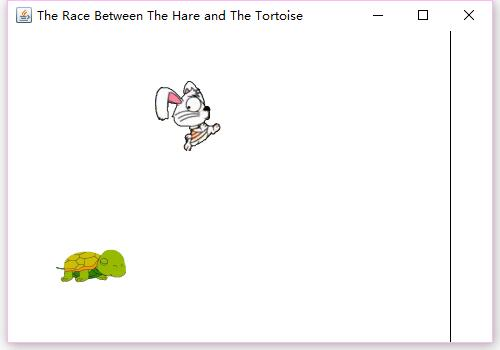
\includegraphics{result1.jpg}
  \end{center}

  \begin{center}
    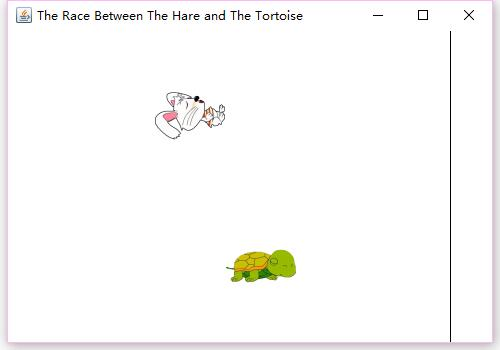
\includegraphics{result2.jpg}
  \end{center}

  \begin{center}
    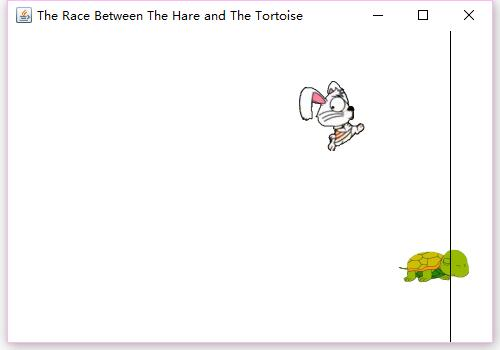
\includegraphics{result3.jpg}
  \end{center}
  
  \newpage

\end{CJK*}
\end{document}
